\subsubsection{Daugiavaizdis konvoliucinis neuroninis tinklas}

Daugiavaizdis konvoliucinis neuroninis tinklas yra aprašytas darbe \cite{cnnExp1}. Daugiavaizdis konvoliucinis neuroninis tinklas - tai konvoliucinis neuroninis tinklas, turintis vieną vaizdų sujungimo sluoksnį (angl. view pooling layer). Vaizdų sujungimo sluoksnis - tai sluoksnis, kuriame kiekvieno duomenų rinkinio požymių žemėlapių rinkiniai, vadinami vaizdais, yra apjungiami. Vaizdų apjungimas yra atliekamas padalinant visus vaizdus į grupes su nurodytu tuo pačiu dydžiu, ir išsirenkant iš kiekvienos grupės po tiksliausią požymių žemėlapių rinkinį.

Daugiavaizdžio konvoliucinio neuroninio tinklo apmokymas vyksta dvejais etapais. Pirmasis etapas yra pasirinkto konvoliucinio neuroninio tinklo apmokymas. Tada antrasis etapas yra vaizdų apjungimo sluoksnio įterpimas ir apmokymo pratęsimas. Šis sluoksnis padalina apmokytą konvoliucinį neuroninį tinklą į du tinklus $C_1$ ir $C_2$. Tęsiant apmokymą, kiekviena 2D nuotrauka atskirai pereis $C_1$ tinklą. Tada vaizdų apjungimo sluoksnyje šios nuotraukos bus apjungiamos. Pabaigoje vaizdų apjungimo sluoksnio rezultatas pereis tinklą $C_2$. Daugiavaizdis konvoliucinis neuroninis tinklas yra atvaizduotas \ref{img:mvcnn} paveikslėlyje.

\begin{figure}[H]
	\centering
	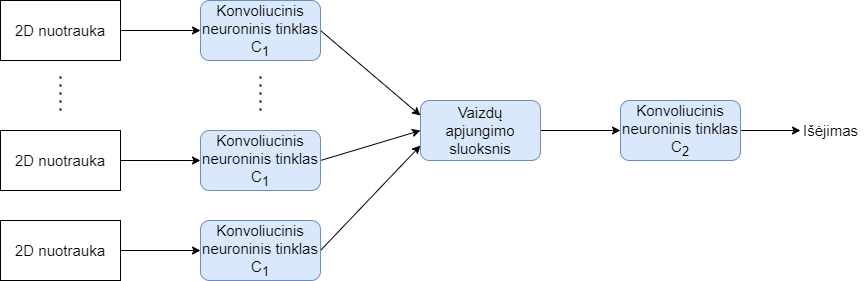
\includegraphics[scale=0.5]{img/mvcnn.png}
	\caption{Daugiavaizdis konvoliucinis neuroninis tinklas}
	\label{img:mvcnn}
\end{figure}

Darbo \cite{cnnExp1} autoriai teigia, kad teoriškai vaizdų apjungimo sluoksnį galima įterpti į bet kurią apmokyto konvoliucinio tinklo vietą. Tačiau tame darbe atlikti tyrimai parodė, kad didžiausias tikslumas yra pasiekiamas įterpus šį sluoksnį šalia paskutinio konvoliucijos sluoksnio.

Darbe \cite{cnnExp1} aprašytas daugiavaizdis konvoliucinis neuroninis tinklas pirmame apmokymo etape naudoja VGG-M architektūra, kuri yra aprašyta darbe \cite{vggM}. Tačiau darbe \cite{cnnExp2} yra pasirinkta VGG-11 architektūra ir darbe \cite{cnnExp2} atliktame tyrime  daugiavaizdis konvoliucinis neuroninis tinklas pasiekė šiek tiek geresnius rezultatus. VGG-11 architektūra yra aprašyta darbe \cite{vgg11}. Šios architektūros konfigūracija yra atvaizduota lentelėje \ref{tbl:vgg11}. VGG-11 architektūroje po kiekvieno konvoliucijos ir pilnai sujungto sluoksnio, išskyrus paskutinio, tolimesnis sluoksnis yra apjungtas netiesiškumo ir ištaisymo sluoksnis su ištaisymo tiesine aktyvacijos funkcija. Tad, tam kad padaryti architektūros atvaizdavimą paprastesnį, šie sluoksniai nėra atvaizduoti lentelėje \ref{tbl:vgg11}. Po paskutinio pilnai sujungto sluoksnio tolimesnis sluoksnis yra netiesiškumo sluoksnis su softmax aktyvacijos funkcija. Taip pat šioje architektūroje visų konvoliucinių sluoksnių branduolių matmenys yra 3x3 ir lango žingsnis yra 1. Tuo metu visų sujungimo sluoksnių langų matmenys yra 2x2, lango žingsniai yra 2 ir visi sujungimo sluoksniai naudoja maksimalaus sujungimo metodą. Tad lentelėje \ref{tbl:vgg11} šie parametrai nėra atvaizduojami.

\begin{table}[h]
	\begin{tabular}{|l|c|l|}
		\hline
		Sluoksnio žymėjimas & Sluoksnio tipas            & \multicolumn{1}{c|}{Parametrai}       \\ \hline
		& Įėjimo sluoksnis           & Įėjimo matmenys = 224x224 RGB matrica \\ \hline
		$c_1$               & Konvoliucijos sluoksnis    & Branduolių skaičius = 64              \\ \hline
		$p_1$               & Sujungimo sluoksnis        &                                       \\ \hline
		$c_1$               & Konvoliucijos sluoksnis    & Branduolių skaičius = 128             \\ \hline
		$p_1$               & Sujungimo sluoksnis        &                                       \\ \hline
		$c_1$               & Konvoliucijos sluoksnis    & Branduolių skaičius = 256             \\ \hline
		$c_1$               & Konvoliucijos sluoksnis    & Branduolių skaičius = 256             \\ \hline
		$p_1$               & Sujungimo sluoksnis        &                                       \\ \hline
		$c_1$               & Konvoliucijos sluoksnis    & Branduolių skaičius = 512             \\ \hline
		$c_1$               & Konvoliucijos sluoksnis    & Branduolių skaičius = 512             \\ \hline
		$p_1$               & Sujungimo sluoksnis        &                                       \\ \hline
		$c_1$               & Konvoliucijos sluoksnis    & Branduolių skaičius = 512             \\ \hline
		$c_1$               & Konvoliucijos sluoksnis    & Branduolių skaičius = 512             \\ \hline
		$p_1$               & Sujungimo sluoksnis        &                                       \\ \hline
		$fc_1$              & Pilnai sujungtas sluoksnis & Neuronų skaičius = 4096               \\ \hline
		$fc_1$              & Pilnai sujungtas sluoksnis & Neuronų skaičius = 4096               \\ \hline
		$fc_1$              & Pilnai sujungtas sluoksnis & Neuronų skaičius = 1000               \\ \hline
		$fc_1$              & Pilnai sujungtas sluoksnis & Aktyvacijos funkcija - softmax        \\ \hline
	\end{tabular}
	\caption{VGG-11 architektūra}
	\label{tbl:vgg11}
\end{table}

Pirmame ir antrame apmokymo etape yra optimizuojama kryžminės entropijos nuostolių funkcija naudojantis Adam optimizavimo algoritmu. Antro etapo pradžioje vaizdų apjungimo sluoksnis yra įterpiamas tarp sluoksnių $p_5$ ir $fc_1$. Šio sluoksnio vaizdų grupių dydžiai yra lygūs 12.

% more info on research result or maybe write about it in research section?